\documentclass[12pt]{article}
\usepackage[polish]{babel}
\usepackage[T1]{fontenc}
\usepackage{graphicx}
\usepackage{float}
\usepackage{amssymb}
\usepackage{hyperref}
\usepackage{minted}
\usepackage{fancyvrb} 
\usepackage{multirow}
\usepackage{longtable}

\title{Harmonogram}
\author{Kinga Florek, Jakub Popielarz, \\Radosław Mikołajczyk}


\begin{document}

\makeatletter
    \begin{titlepage}
        \begin{center}
            
\includegraphics[scale=0.8]{agh_znk_wbr_rgb_150ppi.jpg}\\ \bigbreak
            {\Huge \bfseries  \@title }\\[2ex] 
            {\large Autorzy: \\ \@author}\\ \bigbreak
            {\large Temat projektu: \\ Orgzly synchronizacja} \\ \bigbreak
            \vspace{8mm}
            {\huge Studio Projektowe 1} \\ \bigbreak
            {\large Wydział Elektrotechniki, Automatyki, Informatyki i Inżynierii Biomedycznej} \\ 
        \end{center}
    \end{titlepage}
\makeatother



%\tableofcontents
\newpage

%chyba tutaj można by zrobić opis co robimy na kiedy, nasz assessment
%Rozpiska sprintow????
\section{Estymaty czasowe}
Korzystając z ilości godzin podanej w syllabusie wyliczyliśmy, że dysponujemy około 202,5 godzinami (czyli 25 dniami roboczymi po 8 godzin każdy).
Jest to jedynie wyliczenie poglądowe, realnie każdy z 3 członków zespołu jest w stanie poświęcić na realizację projektu około 8 dni roboczych po 8 godzin każdy.
\\
Przewidujemy czas trwania projektu do 9.06.2021, by uwzględnić dodatkowy czas potrzebny na przygotowanie do sesji egzaminacyjnej. Dzieląc ten okres na dwutygodniowe sprinty otrzymaliśmy ich 6, z czego pierwszy kończy się 31.03.2021.
\\
W związku z tymi przewidywaniami nie będzie możliwe zaimplementowanie zarówno możliwości synchronizacji z serwerem SSH jak i GoogleDrive. 
\newpage
\section{Harmonogram sprintów}
% Please add the following required packages to your document preamble:
% \usepackage{multirow}
% \usepackage{longtable}
% Note: It may be necessary to compile the document several times to get a multi-page table to line up properly
\begin{center}
\begin{longtable}{|c|c|p{8.5cm}|}
\hline
\multicolumn{1}{|l|}{Sprint} & \multicolumn{1}{l|}{Termin końcowy} & Zadanie \\ \hline
\endfirsthead
%
\endhead
%
\multirow{4}{*}{\textbf{Sprint 1}} & \multirow{4}{*}{\textbf{31.03.2021}} & Stworzenie harmonogramu \\ \cline{3-3} 
 &  & Stworzenie specyfikacji \\ \cline{3-3} 
 &  & Stworzenie wizualizacji \\ \cline{3-3} 
 &  & Stworzenie repozytorum projektu \\ \hline
\multirow{6}{*}{\textbf{Sprint 2}} & \multirow{6}{*}{\textbf{14.04.2021}} & Stworzenie layoutu dla okna połączenia się poprzez SSH z serwerem (screen poglądowy w sekcji dodatki) \\ \cline{3-3} 
 &  & Dodanie przycisków synchronizacji do bocznego menu (screen poglądowy w sekcji dodatki) \\ \cline{3-3} 
 &  & Dodanie przycisku SSH do menu Repositories (screen poglądowy w sekcji dodatki) \\ \cline{3-3} 
 &  & Wstępna, szkieletowa implementacja nawiązania połączenia SFTP \\ \cline{3-3} 
 &  & Przeanalizowanie istniejącego kodu do synchronizacji repozytoriów \\ \cline{3-3} 
 &  & Stworzenie testowego serwera SSH/SFTP \\ \hline
\multirow{5}{*}{\textbf{Sprint 3}} & \multirow{5}{*}{\textbf{28.04.2021}} & Implementacja połączenia SFTP wraz ze wstępną implementacją przesyłania plików \\ \cline{3-3} 
 &  & Integracja UI z metodami połączenia \\ \cline{3-3} 
 &  & Integracja UI z metodami przesyłu plików \\ \cline{3-3} 
 &  & Stworzenie testów jednostkowych \\ \cline{3-3} 
 &  & Implementacja obsługi isniejącego przycisku Delete (okno Repositories) dla połączenia SSH \\ \hline
\multirow{4}{*}{\textbf{Sprint 4}} & \multirow{4}{*}{\textbf{12.05.2021}} & Pełna implementacja połączenia SFTP i przesyłania plików \\ \cline{3-3} 
 &  & Integracja pobranych plików z serwera z aplikacją (wyświetlenie dodanych notatek lub usunięcie) \\ \cline{3-3} 
 &  & Implementacja możliwości autentykacji hasłem z poziomu aplikacji \\ \cline{3-3} 
 &  & Implementacja możliwości synchronizacji plików w kierunku aplikacja - serwer \\ \hline
\multirow{3}{*}{\textbf{Sprint 5}} & \multirow{3}{*}{\textbf{26.05.2021}} & Implementacja możliwości synchronizacji plików w obu kierunkach \\ \cline{3-3} 
 &  & Wstępna implementacja możliwości autentykacji za pomocą klucza \\ \cline{3-3} 
 &  & Integracja stworzonych funkcjonalności z istniejącym UI aplikacji \\ \hline
\multirow{3}{*}{\textbf{Sprint 6}} & \multirow{3}{*}{\textbf{09.06.2021}} & Pełna implementacja autentykacji za pomocą klucza z poziomu aplikacji \\ \cline{3-3} 
 &  & Przeprowadzenie testów "user acceptance" \\ \cline{3-3} 
 &  & Uzupełnienie dokumentacji projektu \\ \hline
\end{longtable}
\end{center}

\section{Dodatki}
\centering{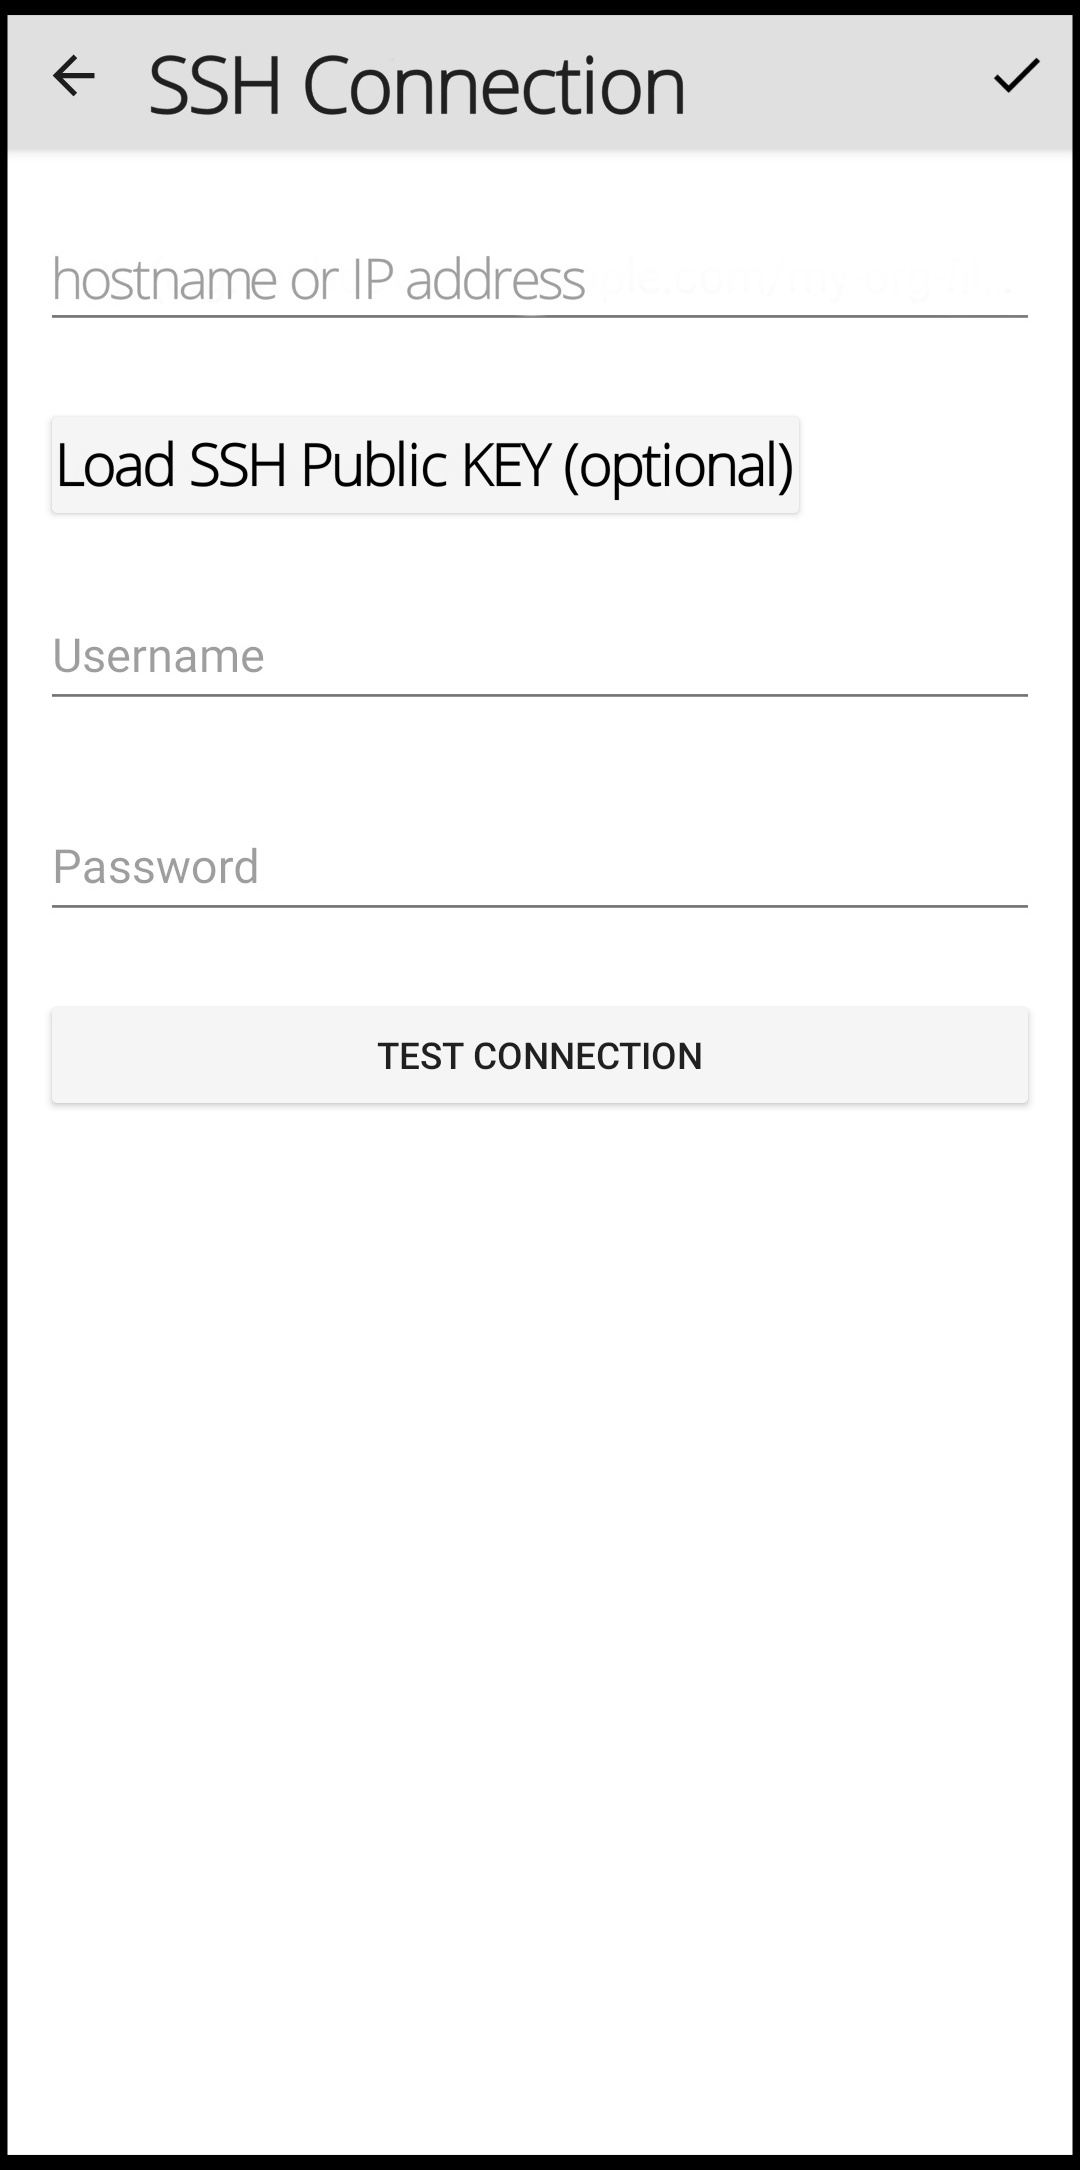
\includegraphics[scale=0.26]{2.jpg} \\
Zdjęcie poglądowe ekranu połączenia się z SSH} \\
\centering{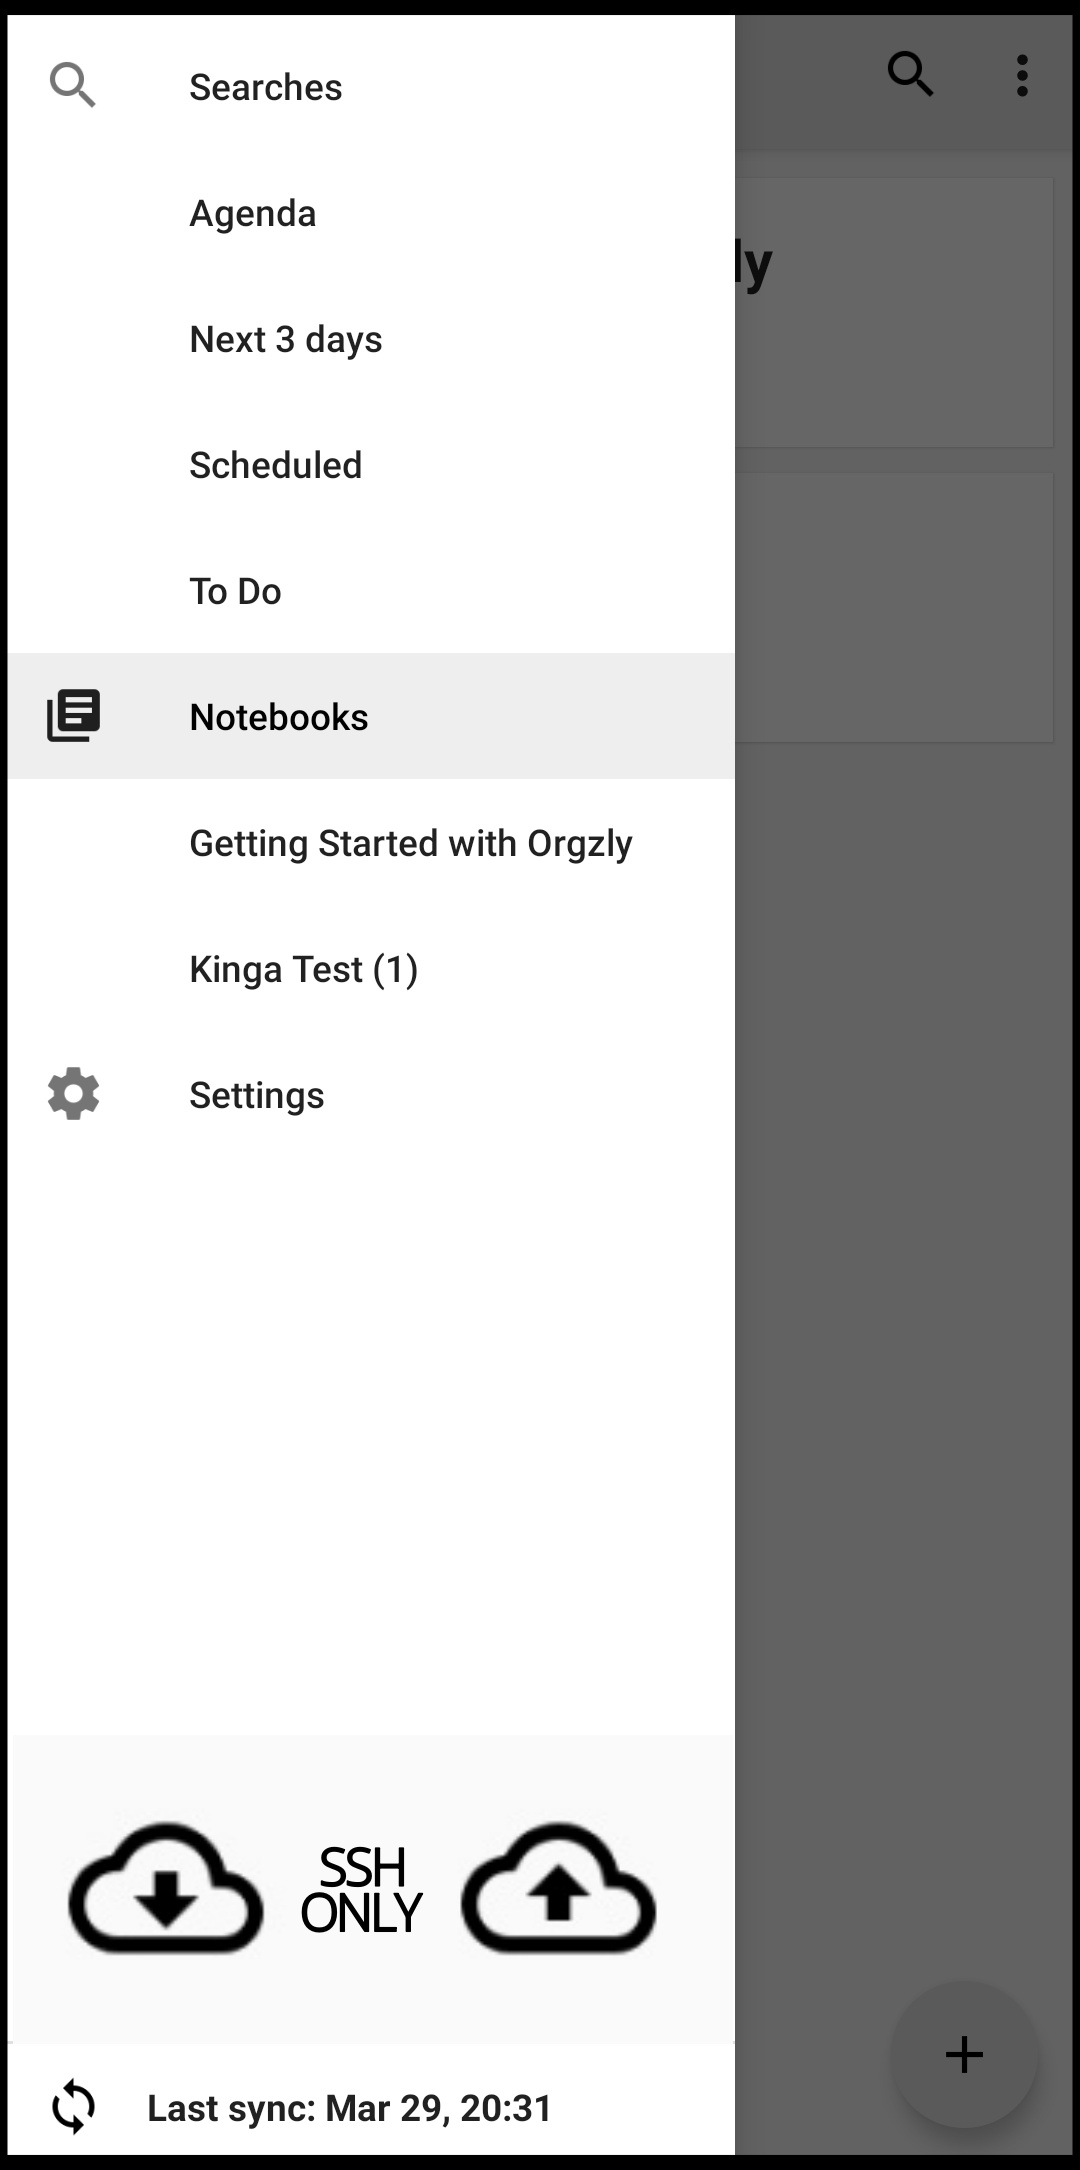
\includegraphics[scale=0.3]{3.jpg} \\
Zdjęcie poglądowe menu, w którym znajdą się przyciski pozwalające na synchronizację plików między serwerem a aplikacją}\\
\centering{ 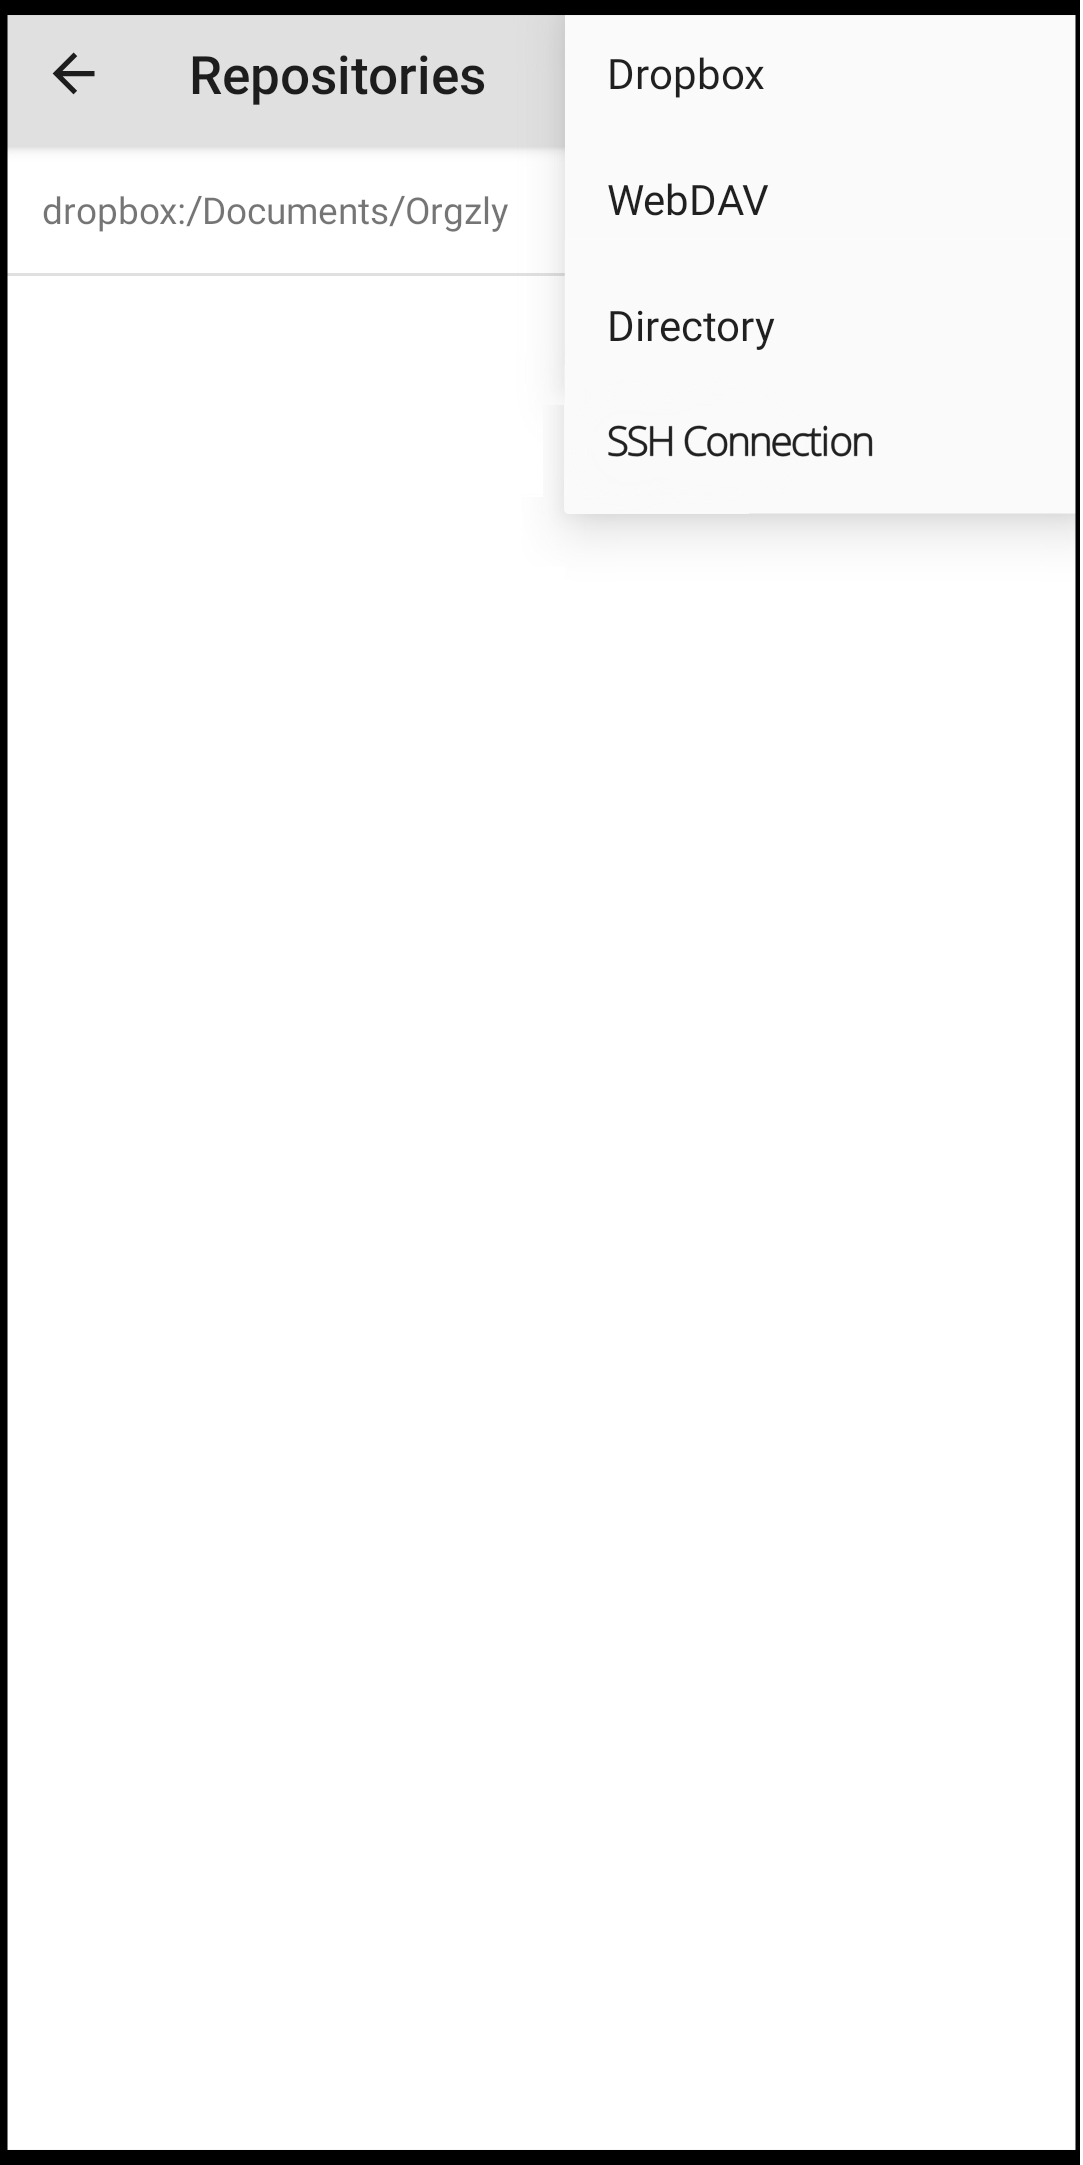
\includegraphics[scale=0.91]{1.png} \\ 
Zdjęcie poglądowe menu Repositories, w którym zostanie dodana opcja SSH Connection}

\end{document}
